\chapter{Estimating the beamline}
\textit{Definition of luminous region, its importance in Alignment and Calibration, luminosity and other stuff}
Definition of luminous region
\begin{figure}
    \centering
    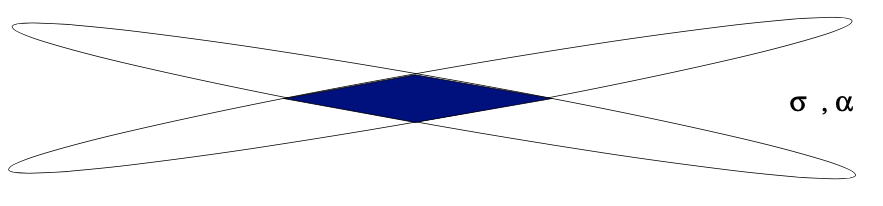
\includegraphics[width=\textwidth]{figures/luminous_region.png}
    \caption{Luminous regions (blue), given the overlap of two bunches}
    \label{fig:luminous-region}
\end{figure}

\begin{figure}
    \centering
    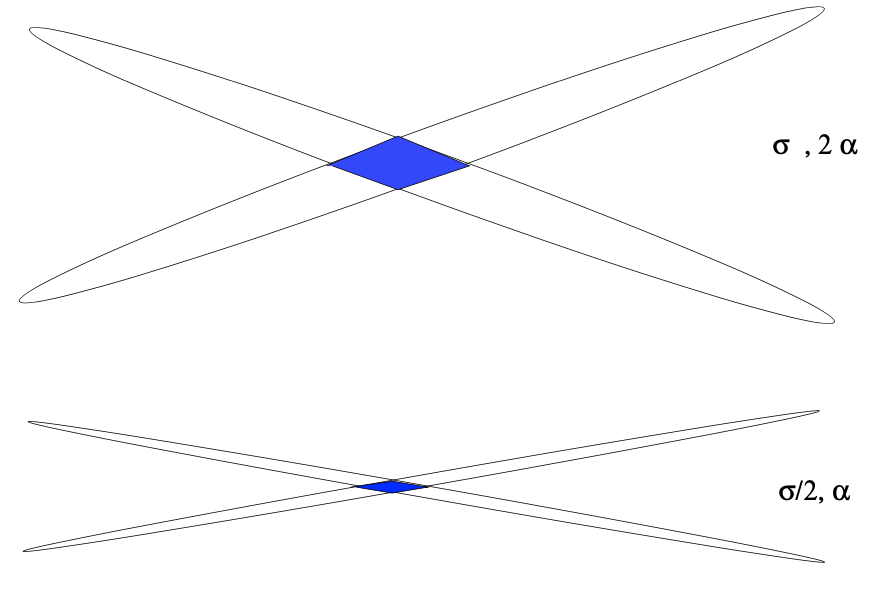
\includegraphics[width=\textwidth]{figures/luminous_region_var.png}
    \caption{Luminous regions (blue), given the overlap of two bunches with different parameters (width \sigma and crossing angle \alpha) with respect to Figure \ref{fig:luminous-region}}
    \label{fig:luminous-region-var}
\end{figure}

\section{Current beamline estimation at LHCb}
\textit{How is the beam now calculated, description of the iterative procedure done during Alignment \& Calibration}

Description of BeamSpot Monitor and the reconstruction performed at HLT1

\section{The Principal Component Analysis}
\textit{Theoretical description of the PCA}

\begin{figure}
    \centering
    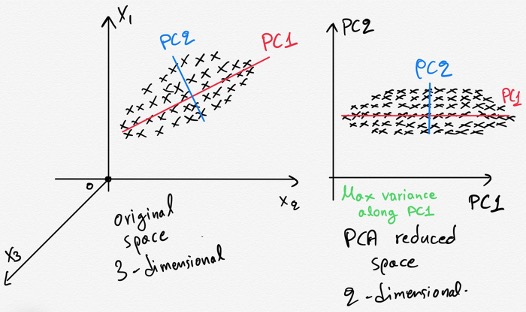
\includegraphics[width=0.8\textwidth]{figures/pca.jpg}
    \caption{Schematic understanding of the Principal Component Analysis}
    \label{fig:pca}
\end{figure}


\section{Monte Carlo simulations}
\textit{Description of the MC simulations available and the results on MC}

\begin{figure}
    \centering
    \begin{subfigure}{0.48\textwidth}
    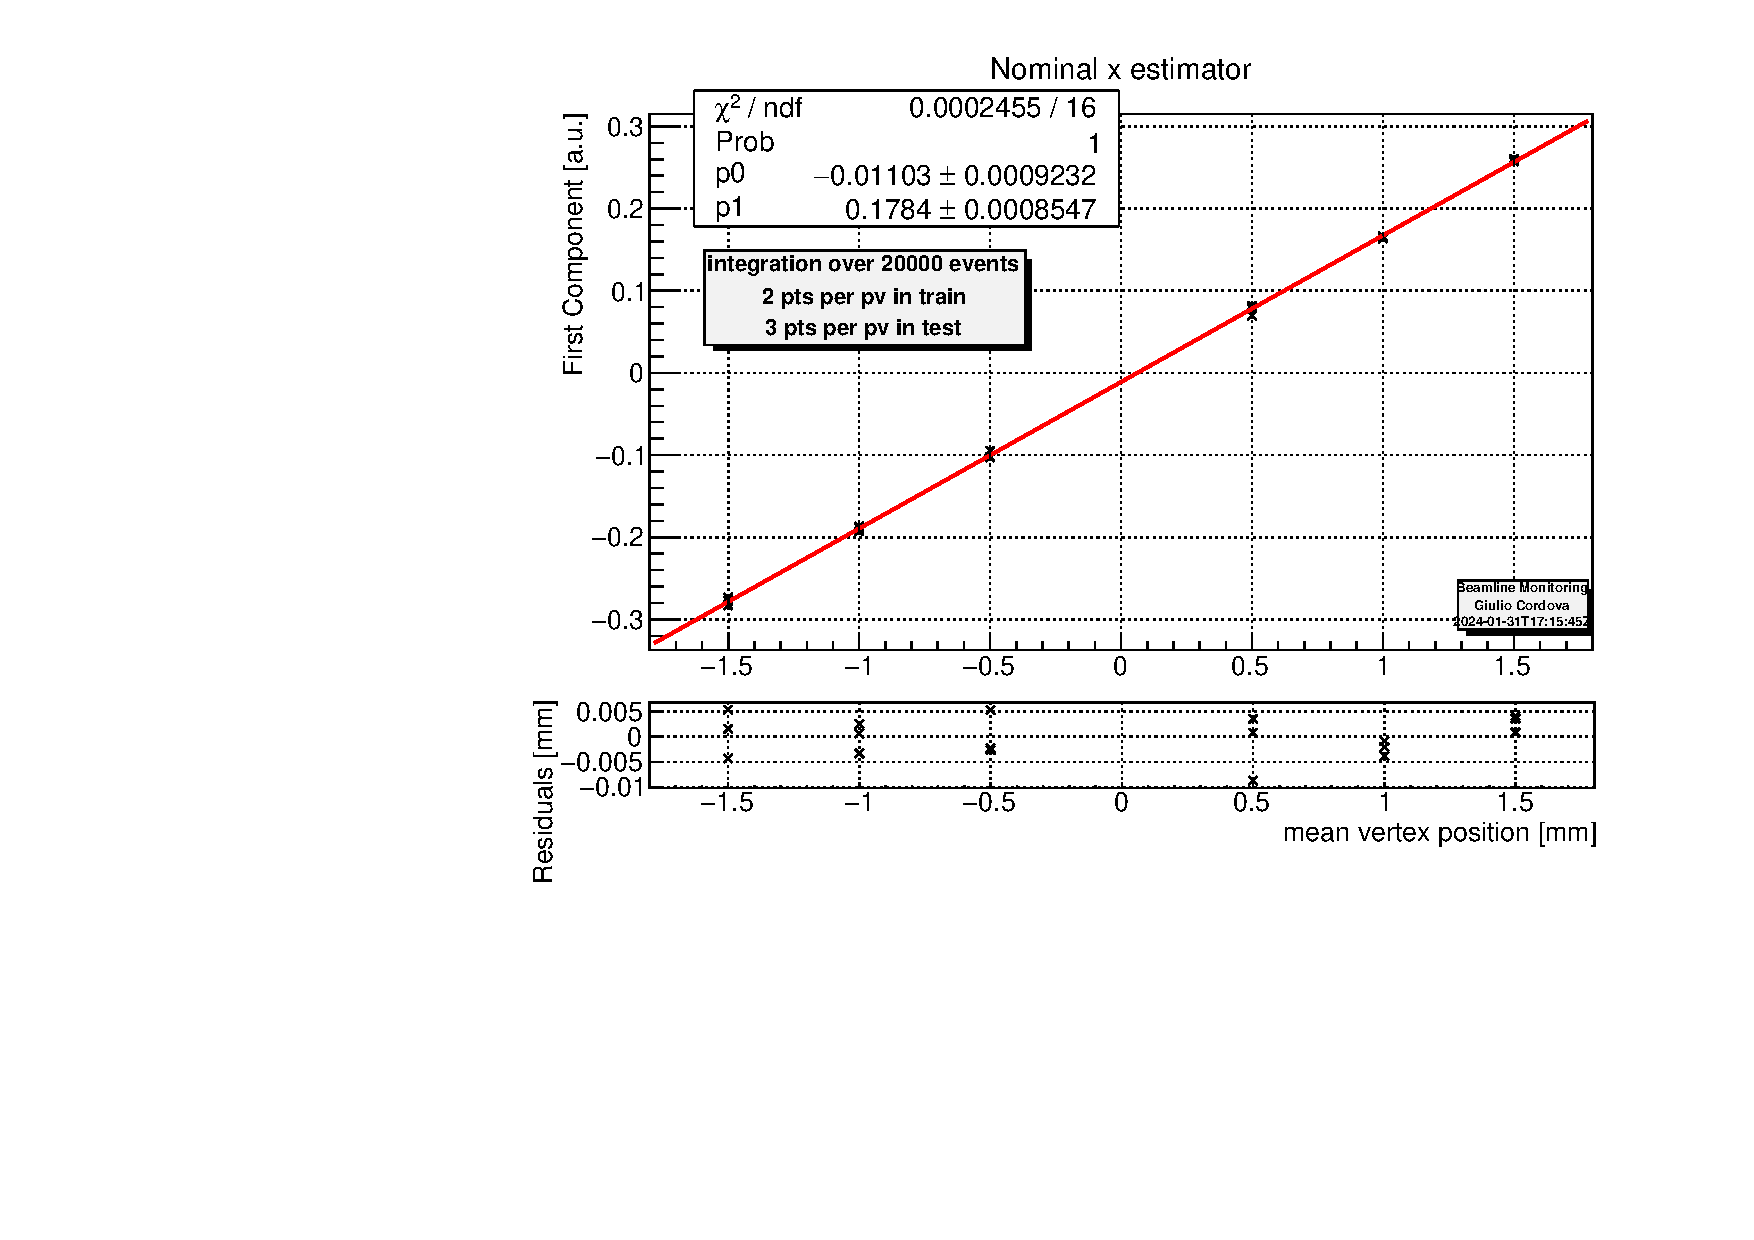
\includegraphics[width=\linewidth]{figures/x_fit.pdf}
    \caption{Linear Fit}\label{fig:xfit_MC}
    \end{subfigure}
    \begin{subfigure}{0.48\textwidth}
    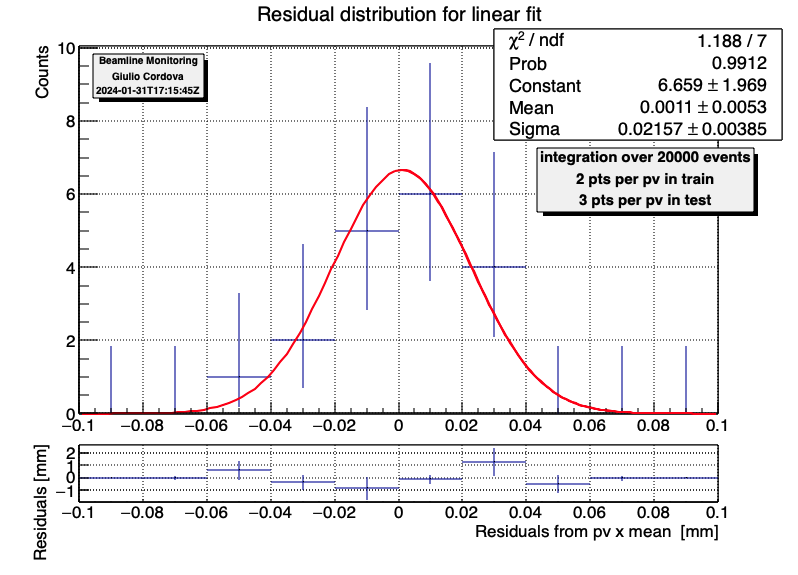
\includegraphics[width=\linewidth]{figures/x_res.png}
    \caption{Residuals from the fit}\label{fig:xres_Mc}
    \end{subfigure}
    \caption{Linearity of the first component calculated with the PCA with respect to beamline position shifts in x component}
    \label{fig:x_MC}
\end{figure}


\begin{figure}
    \centering
    \begin{subfigure}{0.48\textwidth}
    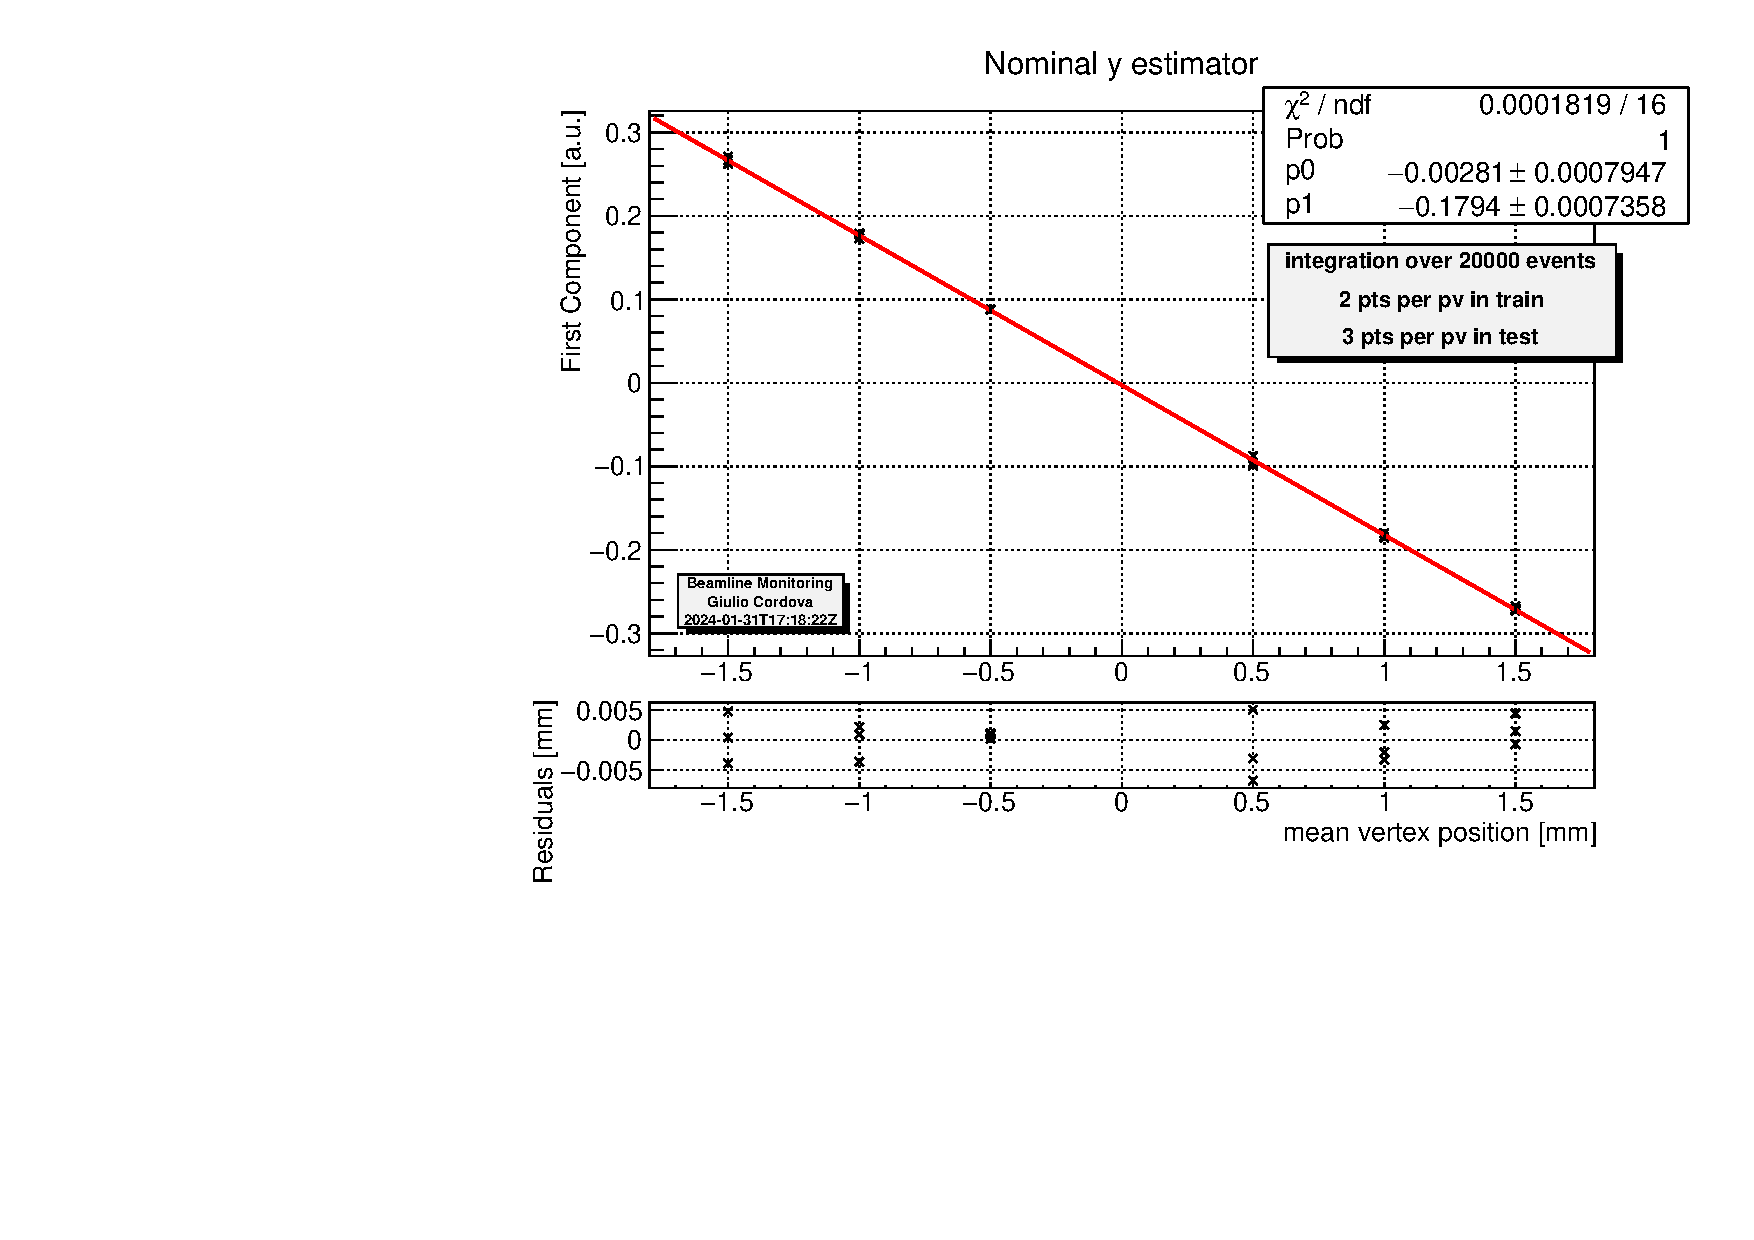
\includegraphics[width=\linewidth]{figures/y_fit.pdf}
    \caption{Linear Fit}\label{fig:yfit_MC}
    \end{subfigure}
    \begin{subfigure}{0.48\textwidth}
    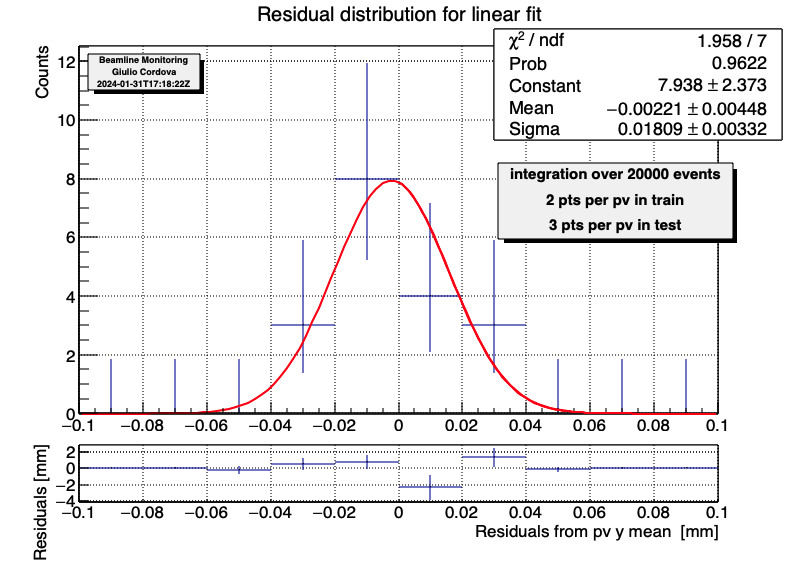
\includegraphics[width=\linewidth]{figures/y_res.png}
    \caption{Residuals from the fit}\label{fig:yres_MC}
    \end{subfigure}
    \caption{Linearity of the first component calculated with the PCA with respect to beamline position shifts in y component}
    \label{fig:y_MC}
\end{figure}


\begin{figure}
    \centering
    \begin{subfigure}{0.48\textwidth}
    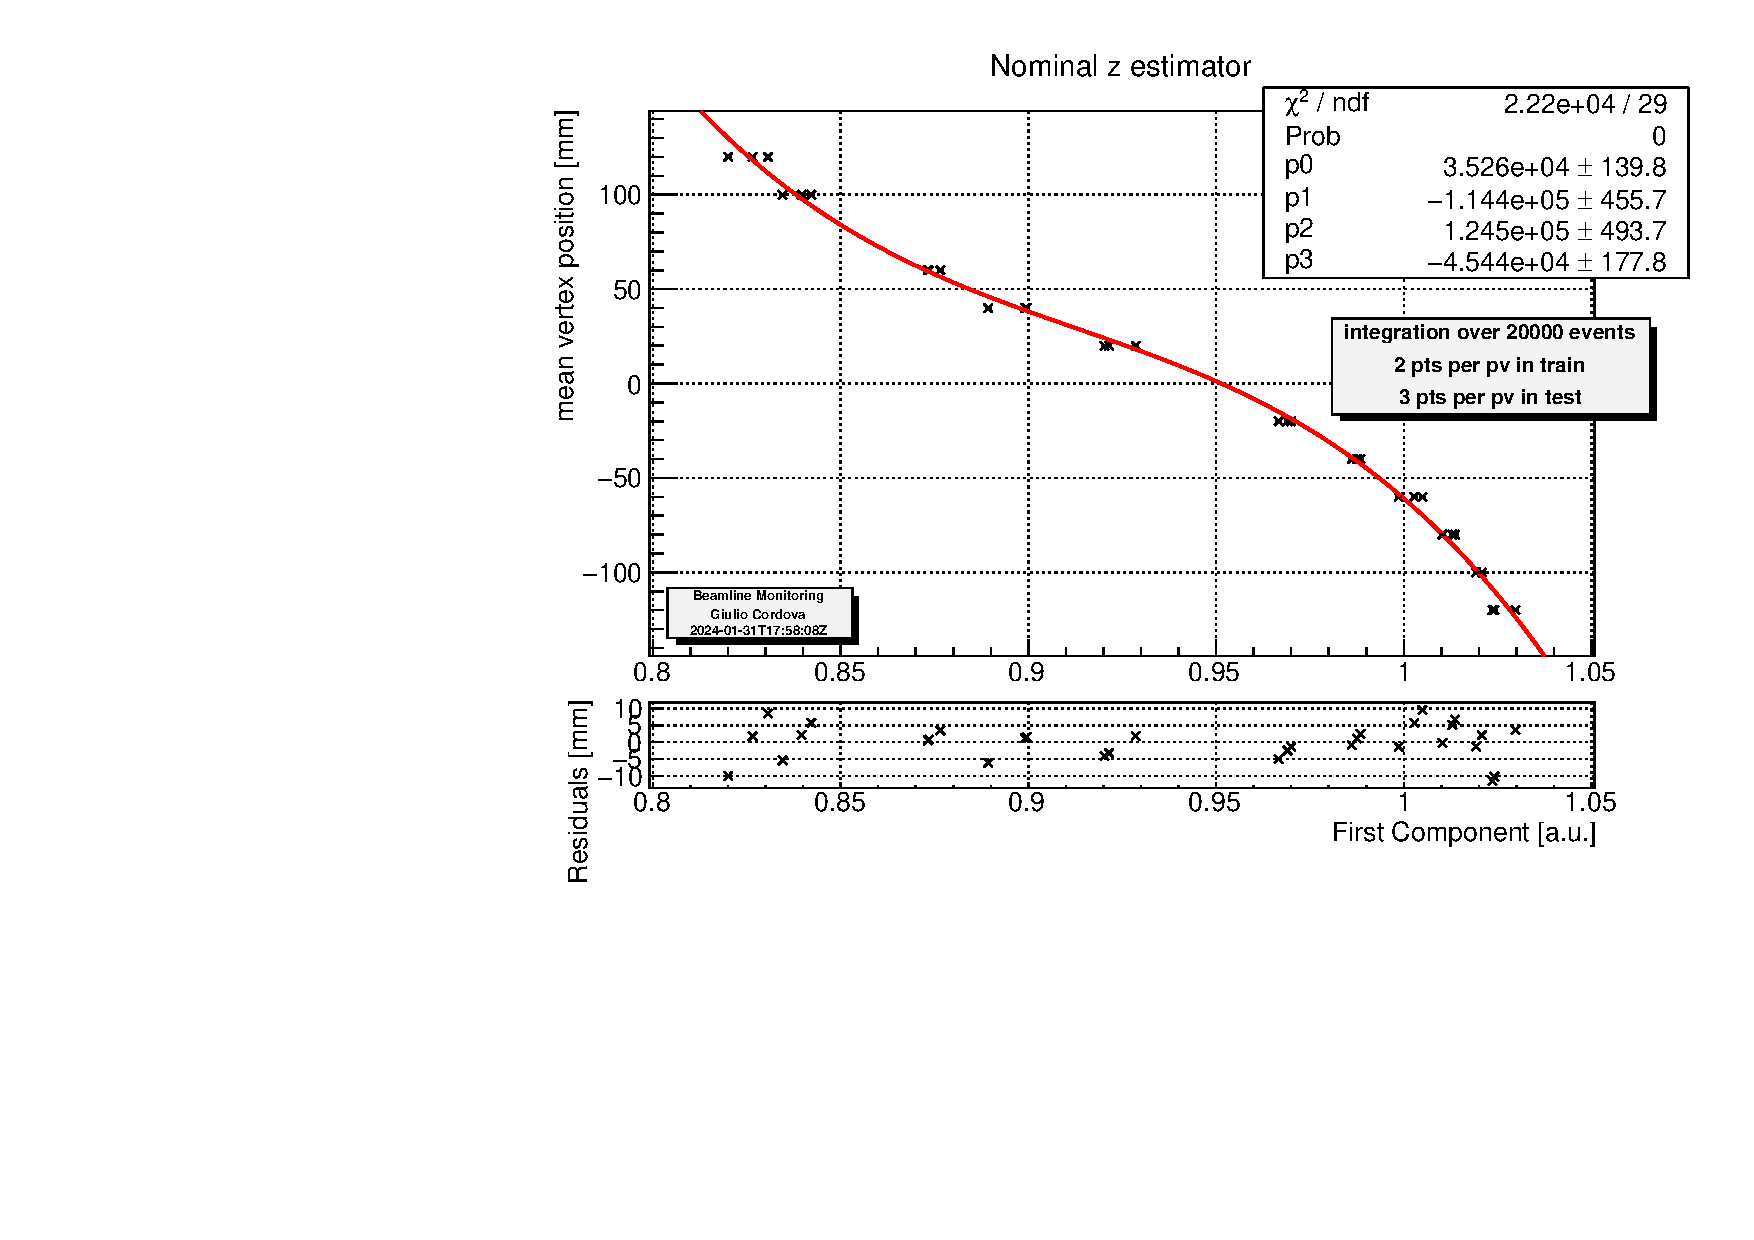
\includegraphics[width=\linewidth]{figures/z_cubic_fit.pdf}
    \caption{Cubic Fit}\label{fig:zfit_cubic_MC}
    \end{subfigure}
    \begin{subfigure}{0.48\textwidth}
    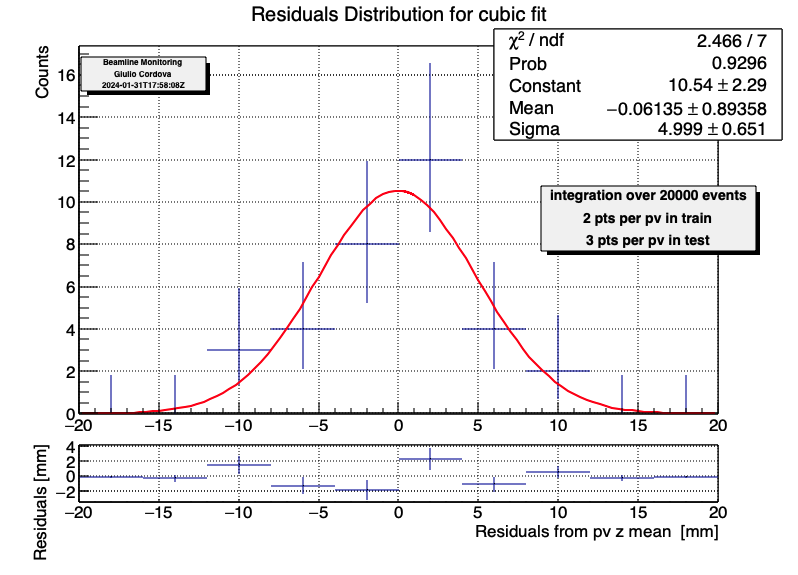
\includegraphics[width=\linewidth]{figures/z_cubic_res.png}
    \caption{Residuals from the fit}\label{fig:zres_cubic_MC}
    \end{subfigure}
    \caption{Cubic relationship between the first component calculated with the PCA and beamline position shifts in z component}
    \label{fig:y_MC}
\end{figure}



\begin{figure}
    \centering
    \begin{subfigure}{0.48\textwidth}
    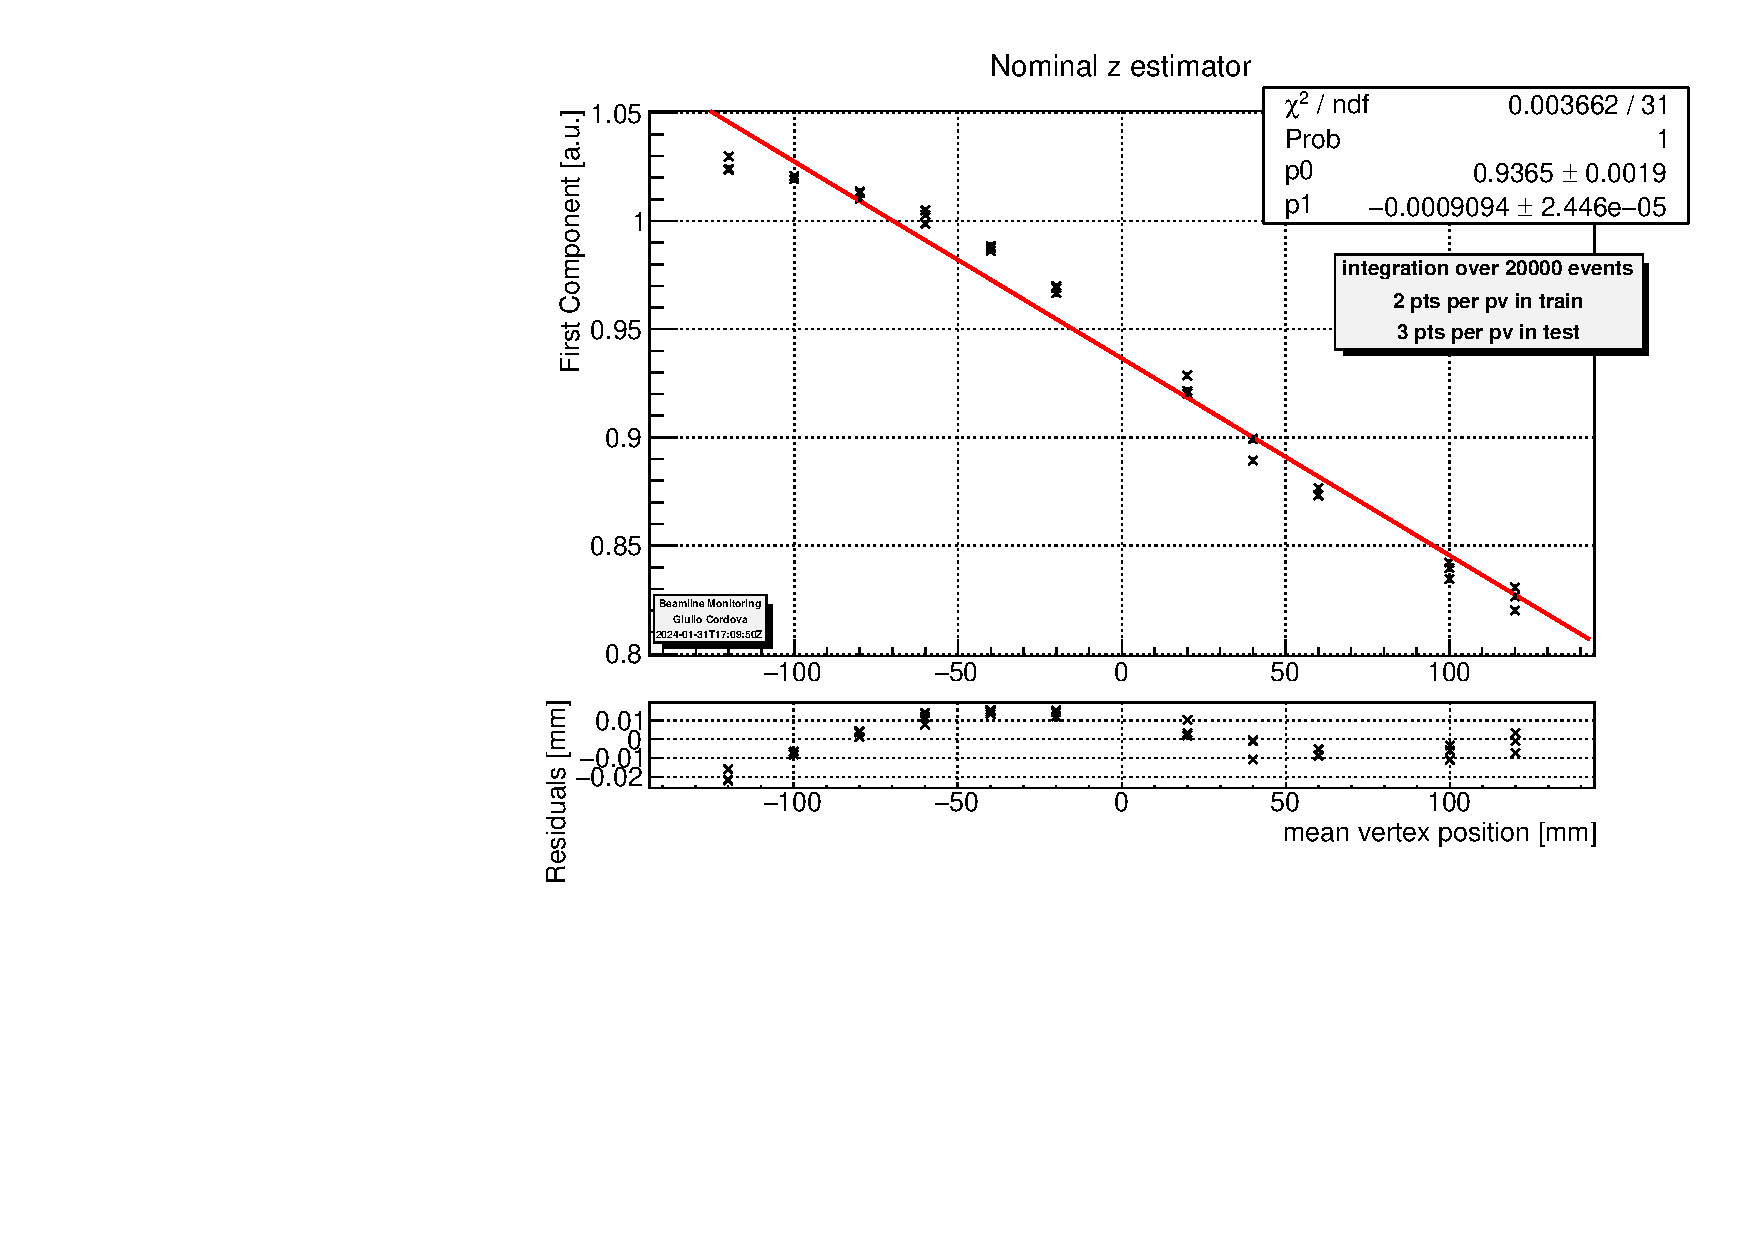
\includegraphics[width=\linewidth]{figures/z_fit.pdf}
    \caption{Linear Fit}\label{fig:zfit_MC}
    \end{subfigure}
    \begin{subfigure}{0.48\textwidth}
    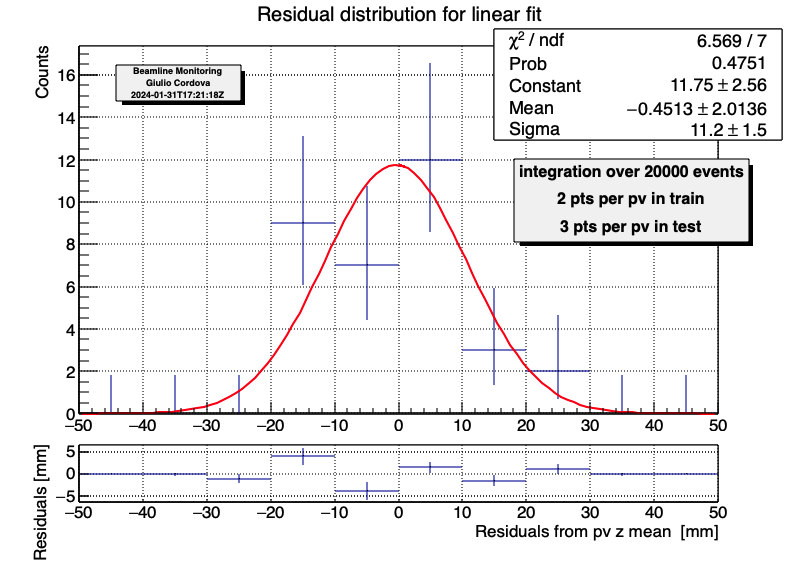
\includegraphics[width=\linewidth]{figures/z_res.png}
    \caption{Residuals from the fit}\label{fig:zres_MC}
    \end{subfigure}
    \caption{Linearity of the first component calculated with the PCA with respect to beamline position shifts in z component}
    \label{fig:z_MC}
\end{figure}


\section{Test on collision data}
\textit{Results obtained during VdM}

\section{Integration in LHCb online system}
\textit{qua ci metto i plot che si vedono nella pagina di Monet e spiego come li abbiamo implementati}
